\section{Rešitev}
Poglejmo si najprej kako izgleda matrika $A_{(n'm')(nm)}$.
\begin{figure}[h]
    \centering
    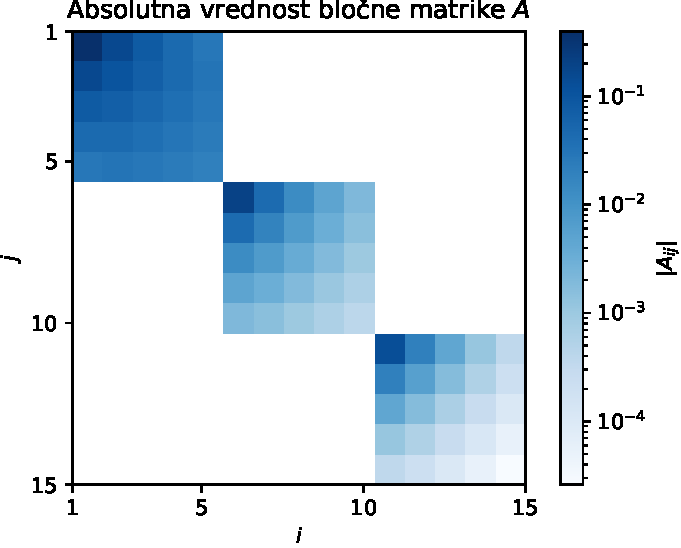
\includegraphics[width=0.8\textwidth]{pdf/A.pdf}
    \caption{Vizualizacija matrike $A_{(n'm')(nm)}$}
\end{figure}

Kako pa izgleda dejansko profil cevi?
\begin{figure}[h]
    \centering
    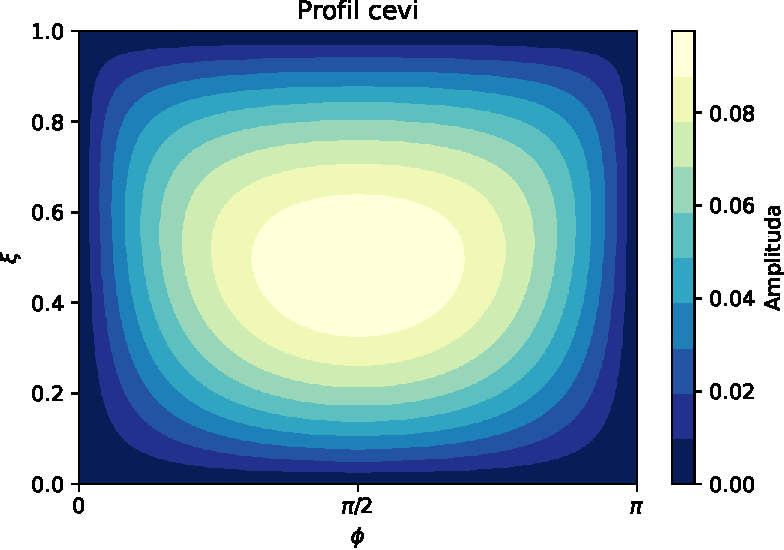
\includegraphics[width=0.48\textwidth]{pdf/cev.pdf}
    \hfill
    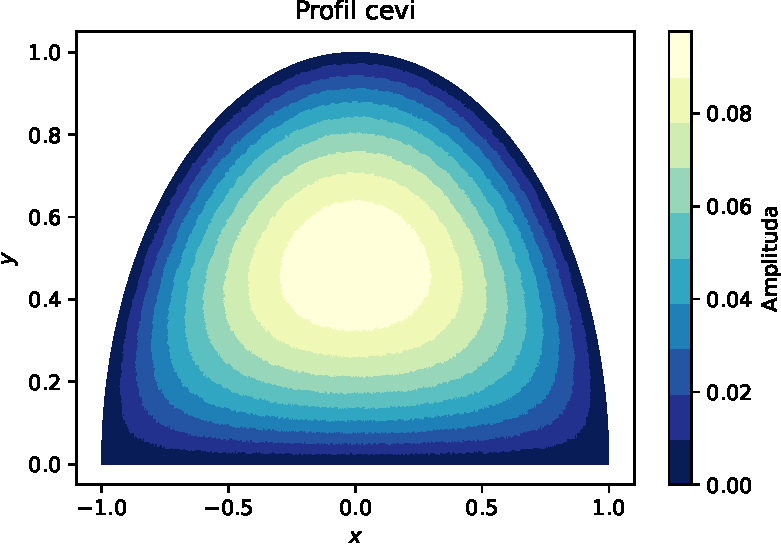
\includegraphics[width=0.48\textwidth]{pdf/cev1.pdf}
    \caption{Profil cevi}
\end{figure}
\newpage
Poglejmo si še časovno odvisnost za izračun C.
\begin{figure}[h]
    \centering
    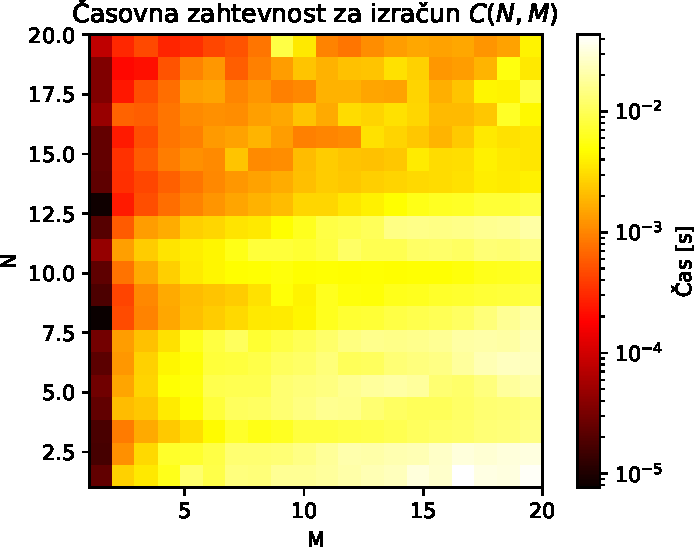
\includegraphics[width=0.5\textwidth]{pdf/time(N,M).pdf}
    \caption{Časovna odvisnost za izračun C}
\end{figure}
Vidimo, da se nam časovno splača hitreje višati $N$ kot $M$.
Poglejmo si še napake v odvisnosti od $N$ in $M$, če rečemo, da je prava rešitev v spodnjem desnem kotu.
\begin{figure}[h]
    \centering
    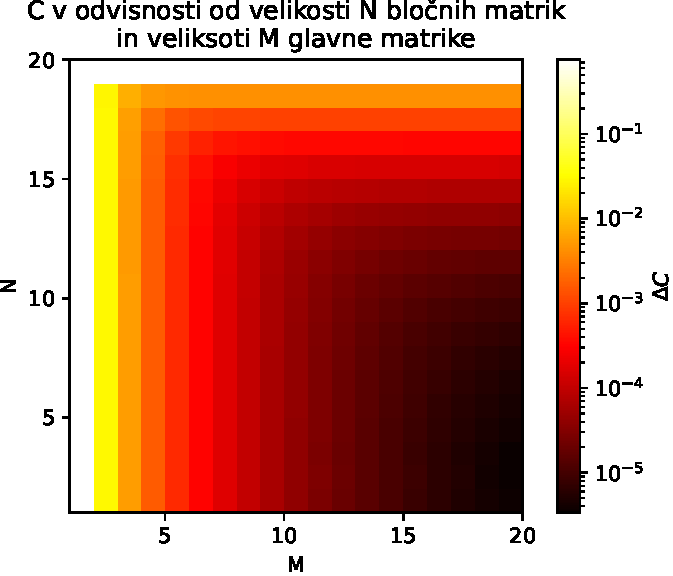
\includegraphics[width=0.5\textwidth]{pdf/C(N,M).pdf}
    \caption{Napaka v odvisnosti od $N$ in $M$ 2d}
\end{figure}
Iz te slike pa ni najbolj razvidno, iz katere strani se bolj splača privliževati.
\newpage
Poglejmo si zato malo bolj podrobneje kako se napaka spreminja z $N$ in $M$.
\begin{figure}[h]
    \centering
    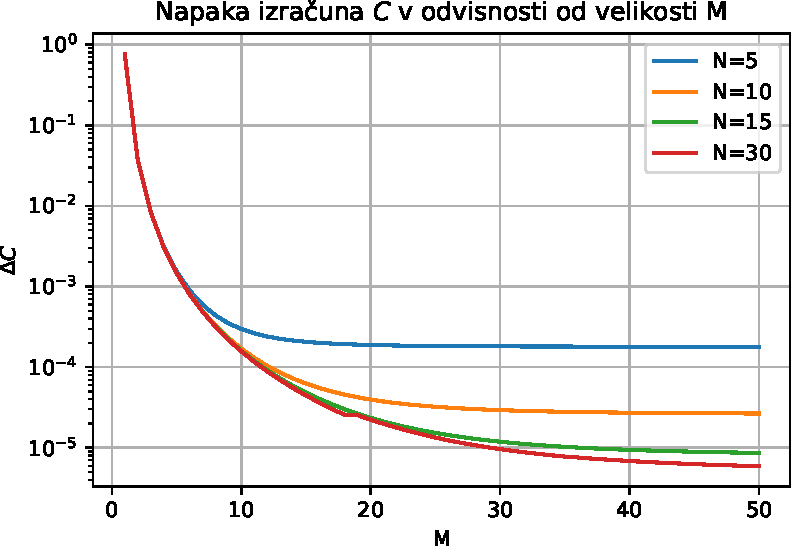
\includegraphics[width=0.6\textwidth]{pdf/C(M).pdf}
    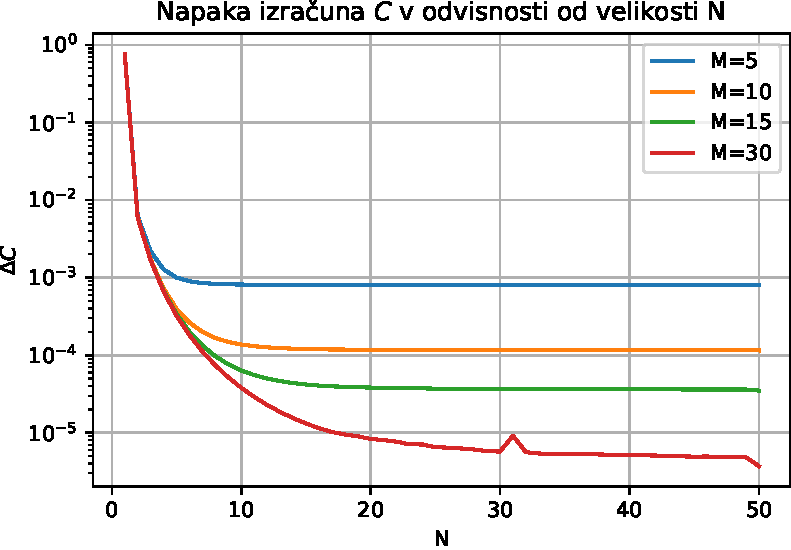
\includegraphics[width=0.6\textwidth]{pdf/C(N).pdf}
    \caption{Napaka v odvisnosti od $M$ in $N$ 1d}
\end{figure}
\newpage
Vidimo da se pri fiksni vrednosti $M$ napaka prej konvergira. Poglejmo si še asimpote napak.
\begin{figure}[h]
    \centering
    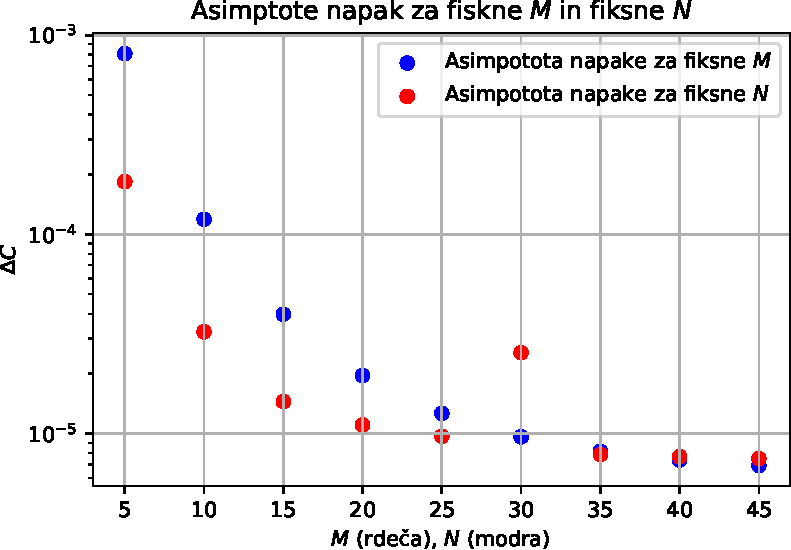
\includegraphics[width=0.6\textwidth]{pdf/Asimpotote_napak.pdf}
    \caption{Asimptote napak}
\end{figure}